\chapter{Case: Interaction Design in a Nutshell} \label{chap:case_meta}
The theory, methods and concepts of this book do not only apply to the design of digital products, but to any kind product that is to be used by humans. As an interesting case study you can consider the very collection of inked sheets of pressed cellulose that you are looking at this very moment. Based on the Y model of section \ref{sec:y_model} this chapter is split into sections for every time the development moves into another outer phase. Note that every section ends with an evaluation with potential users.

\section*{Understanding and evaluation of existing material}
The origin of this book can be placed in a casual conversation between computer science students in the faculties coffee room. As the exam to a course in Human Computer Interaction was moving closer, the students were trying to read up on the material, so quite a few of the resulting conversations were complaining about the material for said course and after a few days also generalizing it to material seen from prior HCI courses. From this the problems with the HCI material were identified to be
\begin{itemize}
  \item A lot of the theory is too fluffy, rather than the rigorous and well defined logic of more mathematical courses liked by the students.
  \item There is a massive amount of text, explanations and theory used for trivial ideas.
  \item Examples are interleaved with theory muddying up the theory to learn.
  \item There are too many examples for the same point. 
\end{itemize}
In the same conversations, which can be seen as unstructured interviews, also the following points about the course structure were brought forward
\begin{itemize}
  \item The theory is taught through a single project, meaning you are quickly locked into a single design space. This is in contrast to the massive amount of small focused exercises in the mathematical courses used to get the student to reflect on almost all the theory.
\end{itemize}
The points above were then confirmed in subsequent conversations in the same coffee room, thereby evaluating the understanding gained.

\begin{figure}
  \centering
  \begin{subfigure}{0.48\textwidth}
    \centering
    \todo
    \caption{Experimental System Design (HCI)}
    \label{fig:meta_books_hci}
  \end{subfigure}
  \hspace{0.1em}
  \begin{subfigure}{0.48\textwidth}
    \centering
    \todo
    \caption{Algebra (Mathematics)}
    \label{fig:meta_books_math}
  \end{subfigure}
  \caption[]{Books used as curriculum for different computer science courses.}
  \label{fig:meta_books}
\end{figure}


\section*{Conceptual Design and creation of the pitch}
Confident in having identified the root problems in the provided HCI course literature, there was taken a closer look at the course literature liked by the disgruntled computer science students, as exemplified in figure \ref{fig:meta_books}. Based on the differences observed the main vision for this book spawned into existence

\begin{displayquote}
  \emph{An HCI book that is written exactly like the course books self-published by the mathematics institute of Aarhus University. Concepts and methods will be written in a 'definition - proof' format of formal mathematics. Examples are focused on a single concept and are put into a seperate part of the book. With the examples are also given larger examples showing the interplay of the methods.}
\end{displayquote}

This fundamental vision for the project does not cover the last point on how HCI courses are structured. With another comparison to the approach of teaching mathematics, the vision for the book is extended with the following to make the final product promote a different (and hopefully more successful) approach at teaching interaction design to computer scientists.

\begin{displayquote}
  \emph{The book will contain small and focused exercises, where the data and understanding needed immediately is provided. It also contains cases to be solved as one or two week handins.}
\end{displayquote}

In conversations over lunch the vision was pitched to other computer science students. All response was extremely positive, claiming they really wished such course material existed and was used.

\section*{Envisionment through prototyping}
With already a pretty concrete vision of the project, the methods from section \ref{sec:envisionment} would not be much of use. On the other hand, testing that the core vision above actually is an improvement for the potential users was vital, which is why a low-fidelity prototype of the concept was the next task.

\begin{figure}[h]
  \centering
  \todo
  \caption[]{Computer science student reading in the first prototype}
  \label{fig:meta_prototype1}
\end{figure}


As shown in \ref{fig:meta_prototype1} a few pages of HCI theory was written in the style of mathematical books and printed out. Based on \ref{prin:economic_principle_of_prototyping} and that writing HCI theory in the style of mathematical books were the only thing of interest at first, these pages did not include any examples or exercises, but only theory. This \emph{paper} prototype was put in front of a few computer science students over a cup of coffee and the feedback was overly positive.

\begin{displayquote}
  \emph{Oh, now I finally get that concept!} - Computer Science Student
\end{displayquote}

With the prototype giving a promising outlook on the vision, more efforts were put into properly copying the style of mathematical books. For this all styling was thrown away for the first prototype and from scratch a new \LaTeX document was written. While creating the base of the project the formatting of the front- and backcover, parts and chapters of the mathematics books were copied to the smallest details. The theory was further fleshed out and the next focus was the seperation and interplay between the three parts \emph{theory}, \emph{examples}, and \emph{exercises} by creating a few pages of theory with associated examples and exercises.

\begin{figure}[h]
  \centering
  \begin{subfigure}{0.48\textwidth}
    \centering
    \todo
    \caption{Interaction Design in a Nutshell (HCI)}
    \label{fig:meta_prototype2_hci}
  \end{subfigure}
  \hspace{0.1em}
  \begin{subfigure}{0.48\textwidth}
    \centering
    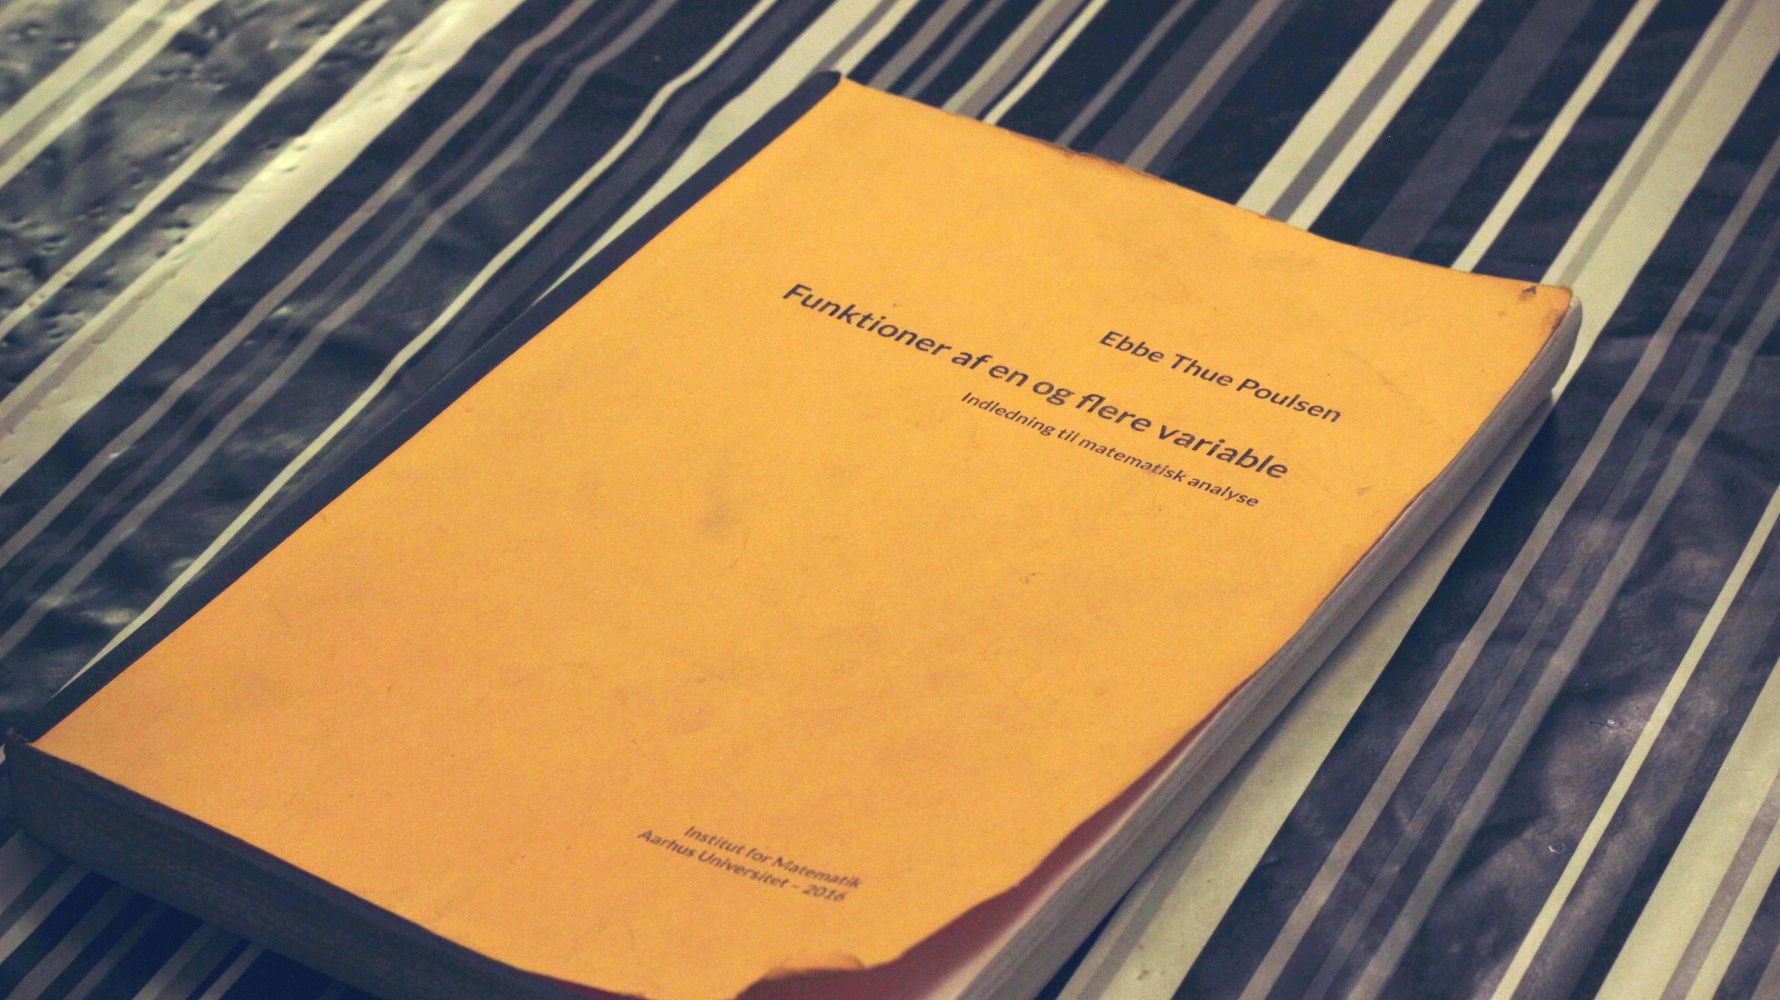
\includegraphics[width=\textwidth]{book_analysis2.jpg}
    \caption{Cover of Mathematical Analysis}
    \label{fig:meta_prototype2_math}
  \end{subfigure}
  \caption[]{(\ref{fig:meta_prototype2_hci}) Second Prototype read by computer student. For comparison there is in \ref{fig:meta_prototype2_math} a book from the faculty of mathematics}
  \label{fig:meta_prototype2}
\end{figure}


\todo




